\section{Weka Decision Tree}
The decision was made early that developing an advanced tree classifier from scratch would
be unnecessary as the Weka 3.6.1\cite{weka} open source library already provided an implementation that meet
all the requirements.  These requirements including being able to classify data sets and 
then being able to query the resulting tree to determine the categorical action based on the set
of non-categorical test.  Also, there was a need to view the resulting tree for visual inspection.

\subsection{Interfacing with Weka}
In order to increase the reusability of the decision tree library, classes were created that 
reproduce the components of the Weka Attribute-Relation File Format (ARFF) instead of merely
storing the contents of an ARFF file.  These classes are of this decision tree library, dtlib, 
are described in the following Table~\ref{table:attribs}.

\begin{table}[h]
\centering
\begin{tabular}{|l|p{5in}|}
\hline
DTAttribute &
Contains two strings representing the name of the attribute and its type.
The type can be either 'numeric' or some enumerated set of the form '\{enum1,enum2,etc\}'.\\
\hline
DTWekaARFF &
Contains a string for the name of the tree, a vector of the non-categorical attributes and the 
categorical attribute as the last element, and a String array representing the data that the 
decision tree will be built from.\\
\hline
DTLearning &
Contains a DTWekaARFF object and a J48 tree object.  The tree object is retrieved by converting
the DTWekaARFF element to the ARFF format and passing it to Weka's 'buildClassifier' function.  
Test are simply a comma separated string of non-categorical data and a '?' for the categorical 
attribute.  The 'DTClassify' method takes this string and creates a proper ARFF format query.
This is then passed to Weka's 'classifyInstance' which returns a double values.  This double value
represents the enumerated string specified in the type of the categorical attribute.  This value is
used to parse the type string and then the appropriate string is returned.  \\
\hline
DTLearningCollection &
Extends Vector to only contain DTLearning objects.\\
\hline
\end{tabular}
\caption{Decicion Tree library classes}
\label{table:attribs}
\end{table}

\subsection{XML declaration}

The decision trees were stored in the configuration XML allowing the behaviour of an agent to be change without
recompiling the entire project.  This flexibility was achieved by structuring the classes so that 
they could be built using the Digester XML parser.  This meant that any decision tree could be modified in 
terms of their non-categorical but the categorical attribute must agree with what is currently within the 
compiled code.  If a new non-categorical attribute was required for a decision tree, then the compiled code would
have to be adapted to know how to retrieve the values of that attribute.

\subsection{Integration with Agent}

The agent contains a class, WekaDT, that contains the constructed decision trees.  This class only has
the necessary methods to retrieve the data necessary to build a test used to query any of the decision
trees.  There is a single private method, 'BuildTest' that will construct test for each tree, this allows the flexibility
of adding non-categorical attributes without adjusting the compiled code.  This method is capable of
examining the current decision tree to determine which non-categorical attributes it contains.

Whenever the agent determines which action to take, it calls the appropriate method for the decision 
tree.  This method calls 'BuildTest' to construct the appropriate which is then queried to the
appropriate tree.  There is then a if-else sequence that based on the returned classified string
will return the proper value.

\subsection{Example}

\begin{figure}[h!]
  \centering  
  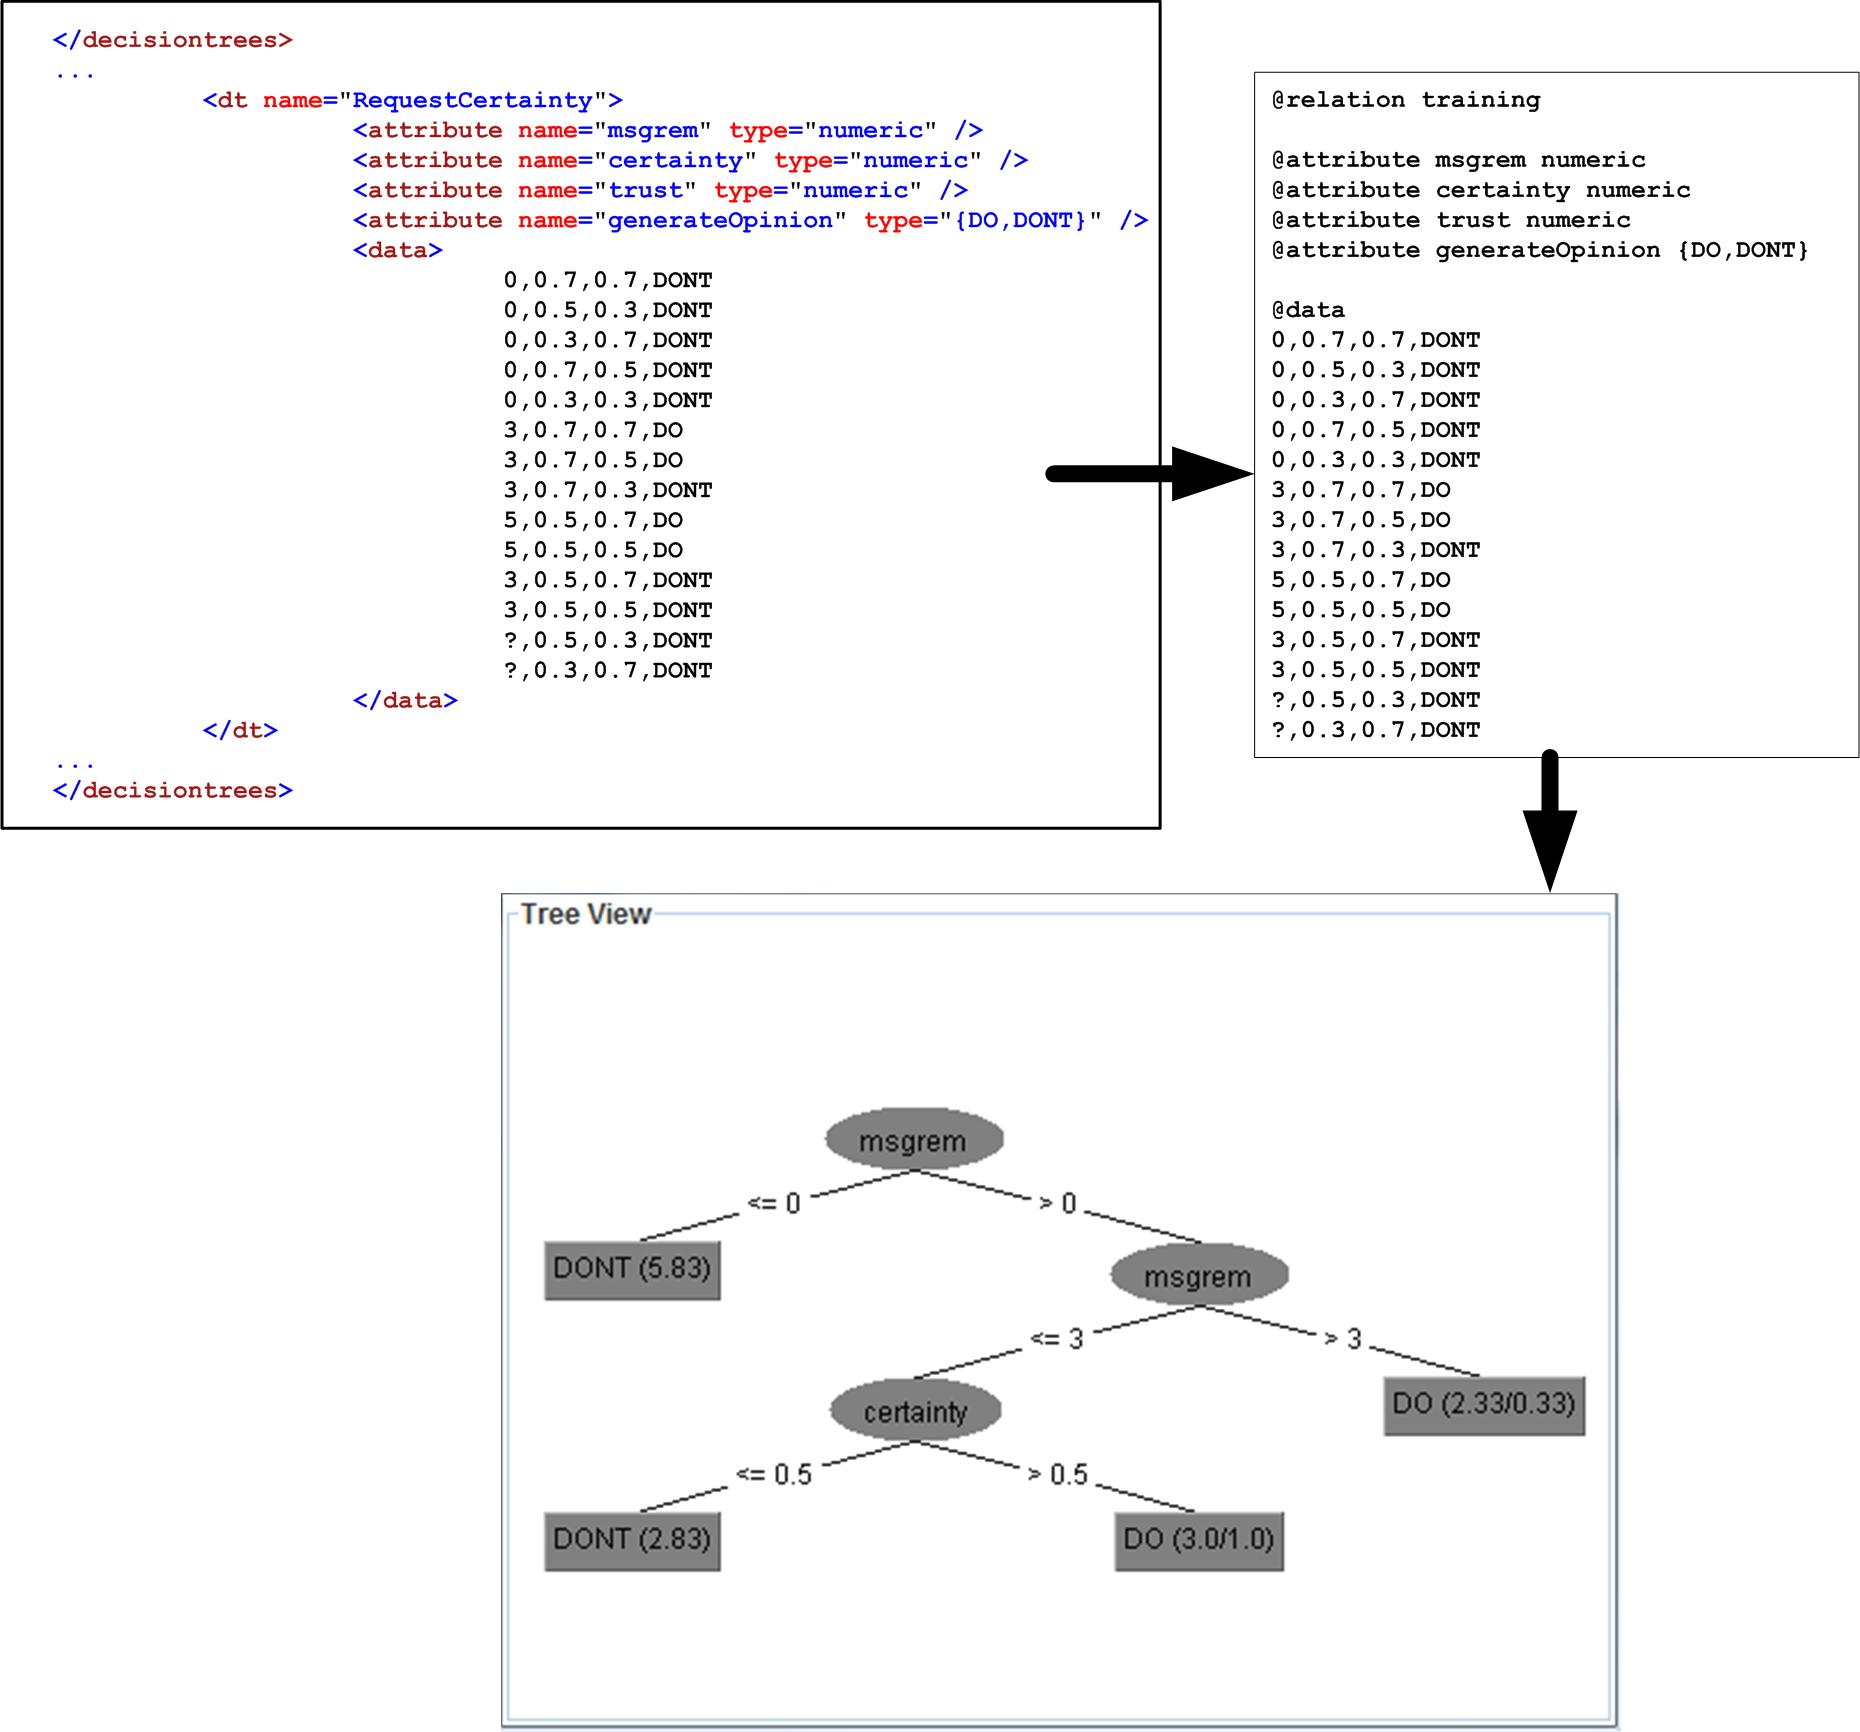
\includegraphics[width=5in]{images/xml2dtxtra.jpg}
  \caption{XML gets converted to the Weka ARFF format and can then be visualized.}
  \label{fig:xml2dt}
\end{figure}

\begin{figure}[h!]
  \centering  
  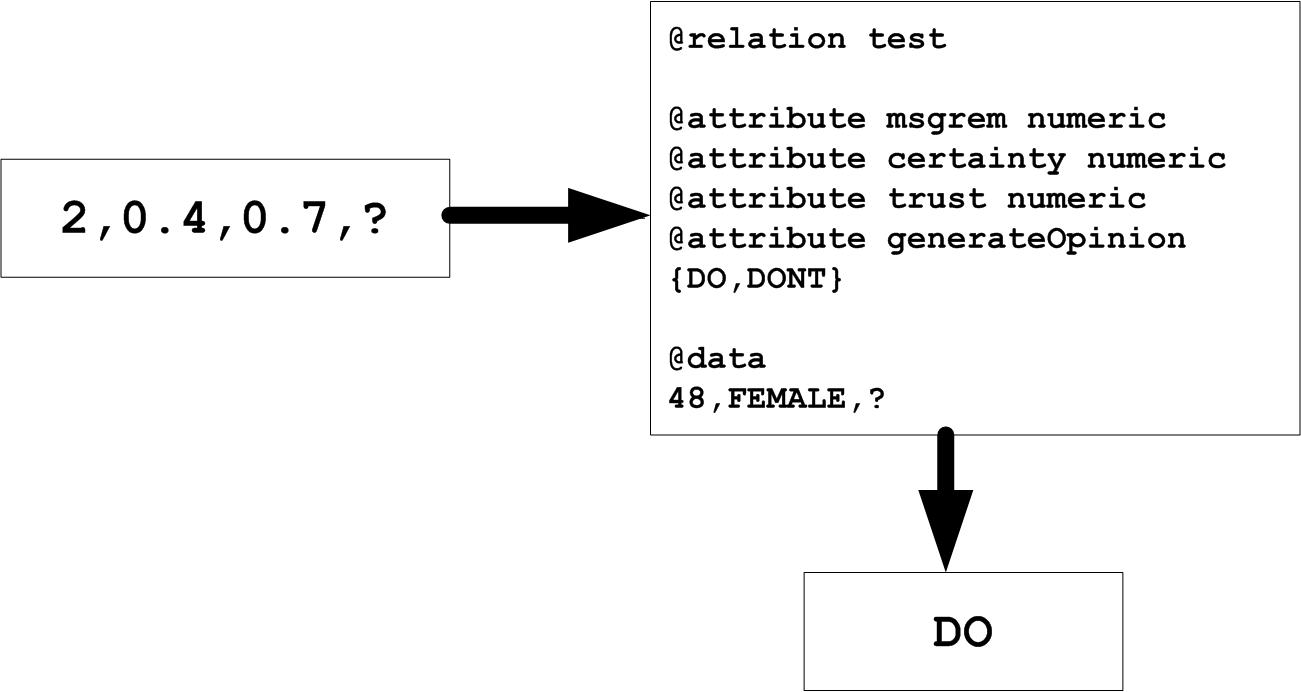
\includegraphics[width=3in]{images/xml2dttest}
  \caption{Comma separated test gets converted to the Weka ARFF format and then gets classified for 
  the tree shown in Figure~\ref{fig:xml2dt}.}
  \label{fig:xml2dttest}
\end{figure}

Figure~\ref{fig:xml2dt} shows a sample decision tree how the shown decision tree can be described in XML.  
In Figure~\ref{fig:xml2dttest} there is a sample comma separated test and its classified return value.

\subsection{Testing and Development of Decision Trees}
Testing was accomplished by first developing a method that opened a Java window and used the Weka
'TreeVisualizer' class to visualize the developed tree.  An application was then written that listed
all the decision trees that were required by the Agent.  Attributes and Data were selected and then 
once the application was run the Weka constructed trees could be visually inspected to ensure that
they met the desired behaviour.

Some workarounds were necessary to properly interface with the Weka library.  Weka functions are
designed to expect Strings of the input file and not simply text reprenting the ARFF format, thus
the DTWekaARFF converted string was then converted to a StringReader which Weka could accept.

The tree classification algorithm used was J48 mainly due its ability to be visualized once constructed.
However, some of the generated trees did not classify data properly resulting in trees that did not
meet the desired behaviour.  By repeating training data entries twice, the J48 algorithm produced
trees that met expected results. 